
\documentclass[a4paper]{article}
% Package fullpage  (réduire les marges)
\usepackage{fullpage}
\usepackage[utf8]{inputenc}
\usepackage[english]{babel}
% \usepackage[left=1.5cm,right=2cm,top=2cm,bottom=2cm]{geometry}


\usepackage{amsmath, amsxtra, amsfonts, amssymb, amstext, amsthm}

\usepackage{booktabs}
\usepackage{fullpage}
\usepackage{nicefrac}
\usepackage{xspace}
\usepackage[noadjust]{cite}
\usepackage{url}\urlstyle{rm}
\usepackage{graphicx}
% \usepackage{graphics}
\usepackage[space]{grffile} 

\usepackage[usenames,dvipsnames]{xcolor}
\usepackage[colorlinks]{hyperref}
\definecolor{linkblue}{rgb}{0.1,0.1,0.8}
\hypersetup{colorlinks=true,linkcolor=linkblue,filecolor=linkblue,urlcolor=linkblue,citecolor=linkblue}
% \usepackage[algo2e,ruled,vlined]{algorithm2e}


\usepackage{wrapfig}
\usepackage{pdfpages}




% --- Code part
\usepackage{listings}
\lstset{language=Python} % Changer eventuellement le nom du langage
\newcommand{\class}[1]{\texttt{#1}}

% --- Math part
\newtheorem{theorem}{Theorem}
\newtheorem{lemma}[theorem]{Lemma}
\newtheorem{proposition}[theorem]{Proposition}
\newtheorem{corollary}[theorem]{Corollary}
\newtheorem{definition}[theorem]{Definition}
\newtheorem{algorithm}[theorem]{Algorithm}
\newtheorem{remark}[theorem]{Remark}



% Mathematic abbreviations

\newcommand{\N}{\mathbb{N}}
\newcommand{\R}{\mathbb{R}}
\newcommand{\Z}{\mathbb{Z}}

\newcommand{\Esp}{\mathbb{E}}
\newcommand{\Prob}{\mathbb{P}}
\newcommand{\Var}{\text{Var}}

\newcommand{\A}{\frak{A}}
\newcommand{\F}{\mathbb{F}}


\renewcommand{\epsilon}{\varepsilon}



% \newcommand{\GF}[1]{\text{GF}(#1)}
\newcommand{\GF}[1]{\F_{#1}}


% More definitions
\usepackage{showkeys}
\usepackage{mathtools}
%\usepackage{multirow}
%\usepackage{appendix}



\author{Sylvain Colin \& Gaspard Férey}
\title{The Sidelnikov-Shestakov's Attack applied to the Chor-Rivest Cryptosystem}

\begin{document}


\maketitle

\begin{abstract}

In this article, we discuss about the Sidelnikov-Shestakov attack on cryptosystems based on Reed-Solomon codes. Then we describe how this algorithm can be used to improve the attack to the Chor-Rivest Cryptosystem proposed by Vaudenay \cite{Vau01}.

\end{abstract}

\section{Introduction}
\label{sec:intro}

The McEliece cryptosystem \cite{NiederH86} was one of the first to use randomization in the encryption process. Indeed, in such a scheme, the encrypter uses a random error to prevent attacks on the codeword. This codeword is then decrypted using an error-correcting code. 
In \cite{NiederH86}, Niederreiter study discusses the best choices of error-correcting codes which can be used in the cryptosystem. He highlights two families of codes : alternant codes
(including for example Goppa codes, which were used first in the McEliece cryptosystem) and GRS (Generalized Reed-Solomon) codes.
Note that this algorithm has never gained much acceptance in the cryptographic community, but is a candidate for "post-quantum cryptography".

In 1992, Sidelnikov and Shestakov suggest an attack \cite{SidelShes92} on the public key of this cryptosystem (based on GRS codes) using equivalences between private keys.

Nowadays, all the versions of the McEliece cryptosystem had been broken.

The Chor-Rivest cryptosystem \cite{ChorRiv88} is a public key knapsack system which has been broken.  However, it took longer to break than most, and is a very elegant use of finite fields.

The first efficient attack for the proposed range of parameters (i.e., $p \simeq 256$, $h \simeq 24$) has been obtained by Vaudenay in 2001, assuming there exists a small factor $r$ of $h$ with $r > \sqrt{h}$.


\subsubsection*{Our Work}
In this article, we first describe the Niederreiter and McEliece cryptosystem and present the original Sidelnikov and Shestakov's attack \cite{SidelShes92}, which is also explained more clearly by Wieschebrink \cite{Wiesch}.
We try to make a mix between the simplicity of the arguments given by Wieshbrink, which lead to a better understanding of the attack, and the generality of the article of Sidelnikov and Shestakov, who introduce a notion of infinity,
not introduced by Wieshbrink, and which leads to get a better complexity.

On a second part, we focus on the Chor-Rivest cryptosystem and show some similarities between the "known $g_{p^r}$ attack" introduced by Vaudenay and the Sidelnikov-Shestakov attack. Indeed, $\F_{p^r}$ can be seen as a $\F_p$-vector space and the knowledge of the particular generator $g_{p^r}$ of $\F_{p^r}$ yield the values of $r$ small degree polynomials in the private key $\alpha_{\pi(j)}$. This was how Vaudenay was able to suggest a "known $g_{p^r}$" attack working for any factor $r$ of $h$ bigger than $\sqrt{h}$.

These similarities allow us to describe a more efficient algorithm for a "known $g_{p^r}$ attack" which require $r$ to be much smaller than in Vaudenay's article. Using the small powers of $g_{p^r}$, we manage to get the weaker condition $r > \log p$. In particular the term $p^{\sqrt{h}}$ in Vaudenay's complexity corresponding to an exhaustive research can be reduced to $p^{\log p}$ assuming we have $h \simeq \frac{p}{\log p}$  and $h$ has very small factors (around $\log p$). The first condition is suggested in Chor and Rivest's article because the density of the  finite field chosen should be close to 1 in order for the cryptosystem not be attacked using lattice reduction algorithms . That last point should be verified since the scheme can only be used efficiently when $h$ has a lot of divisors in order to be able to compute discrete logarithms for the public key.




\section{Preliminaries}
\label{sec:Prel}


\subsection{A cryptosystem based on Reed-Solomon codes}
\subsubsection{Key generation}

We study here the public-key cryptosystem introduced first by Niederreiter and McEliece \cite{NiederH86} and based on generalized Reed-Solomon codes.

Let $\F_q$ be a finite field with $q = p^h$ elements and $\F = \F_q \cup \{ \infty \}$, where $\infty$ has usual properties ( $1/\infty = 0$, etc). We call $G$ the following matrix:
$$ G(\alpha_1, \ ... \ , \alpha_n, z_1, \ ... \ , z_n) := \left(
\begin{array}{cccc}
z_1 \alpha_1^0 &  z_2 \alpha_2^0 & \cdots & z_n \alpha_n^0 \\
z_1 \alpha_1^1 &  z_2 \alpha_2^1 & \cdots & z_n \alpha_n^1 \\
 & & \ddots & \\
z_1 \alpha_1^{k-1} &  z_2 \alpha_2^{k-1} & \cdots & z_n \alpha_n^{k-1}
\end{array}
\right) \in \mathcal{M}_{\F}(k,n) $$
where $\alpha_i \in \F$ and $z_i \in \F_q\backslash\{0\}$ for all $i \in \{1,...,n\}$.
As in the article of Sidelnikov and Shestakov \cite{SidelShes92}, if $\alpha_i=\infty$, the $i$-th column is defined by the vector $z_j(0, \ ... \ , 0,1)^{T}$ since the coefficient $\alpha_i^{k-1}$ dominates all the other coefficients $\alpha_i^{j}$ for $j<k-1$.
So, we concretely manipulate finite coefficients. The codes generated by such matrices are called Generalized Reed-Solomon (GRS) codes.

The cryptosystem is also based on a random nonsingular matrix $H$ of size $k\times k$ with coefficients in $\F_q$. Finally, we call $M$ the matrix of size $k\times n$ defined by $M=H\cdot G(\alpha_1, \ ... \ , \alpha_n, z_1, \ ... \ , z_n)$.
It is clear that $M$ has the following general form :
$$ M := \left(
\begin{array}{cccc}
z_1f_1(\alpha_1) &  z_2f_1(\alpha_2) & \cdots & z_nf_1(\alpha_n) \\
z_1f_2(\alpha_1) &  z_2f_2(\alpha_2) & \cdots & z_nf_2(\alpha_n) \\
 & & \ddots & \\
z_1f_k(\alpha_1) &  z_2f_k(\alpha_2) & \cdots & z_nf_k(\alpha_n) \\
\end{array}
\right)$$
where $f_i$ is a polynomial of degree at most $k-1$.
We can notice that, if $\alpha_i = \infty$, $f_j(\alpha_i)$ is equal to the dominant coefficient of the polynomial $f_j$ for all $1\leq j\leq k$ because the last coefficient of the $i$-th column of $G$ is equal to $z_i$ and the others are equal to $0$.

In the considered cryptosystem, the secret key consists of the set $\{\alpha_1,... ,\alpha_n\}$, the set $\{z_1,... ,z_n\}$ and the random matrix $H$.

The public key is given by the representation of the field $\F_q$ (ie. the polynomial used to define $\F_q$ over $\F_p$), the matrix $M$ and the integer $t=\lfloor\frac{n-k}{2}\rfloor$.

\subsubsection{Encryption and Decryption}
The codewords are then the vectors $c=b\cdot M$ where $b\in\F_q^k$. So, the different codewords have necessarily the following form :

$$c=(z_if_c(\alpha_i))_{1\leq i\leq n}$$ where $f_c$ is a polynomial whose degree is at most $k-1$.
Once again, we can notice that, if $\alpha_i = \infty$, $f_c(\alpha_i)$ is equal to the dominant coefficient of the polynomial $f_c$.

Thus, given a message to send, which is actually a vector $b$ of $\F_q^k$, one will have to transmit the vector $b\cdot M + e$ where $e$ is a random vector of $\F_q^n$ with Hamming weight at most $t=\lfloor\frac{n-k}{2}\rfloor$.
Since a GRS code can correct $\lfloor\frac{n-k}{2}\rfloor$ errors, this property remains true for $M$. Indeed, $b\cdot M$ remains a codeword of the GRS code, since it is the codeword obtained applying the GRS code to $b\cdot H$.
So, in order to decrypt the message, we first compute $b'=b\cdot H$, finding the closest codeword from the received message, using for example the Berlekamp-Welch algorithm.
Then, we compute $b'\cdot H^{-1}$ to get the original message.

However, the original message can not be easily recovered when not knowing the GRS code used in the secret key.

\subsection{Equivalence between Reed-Solomon codes}

Sidelnikov and Shestakov show \cite{SidelShes92} that for all $a \in \F_q\backslash\{0\}$ and $b \in \F_q$, there exists $H_1, H_2, H_3 \in \mathcal{M}_{\F_q}(k,k)$ nonsingular, $(c_1,... ,c_n) \in \F_q\backslash\{0\}^{n}$ and $(d_1,... ,d_n) \in \F_q\backslash\{0\}^{n}$ such that:
\begin{equation}
H_1\cdot G(a\cdot\alpha_1 + b, \ ... \ , a\cdot \alpha_n + b, c_1z_1, \ ... \ , c_n z_n) = G(\alpha_1, \ ... \ , \alpha_n, z_1, \ ... \ , z_n)
\label{eq1}
\end{equation}
\begin{equation}
H_2\cdot G\left( \frac{1}{\alpha_1}, \ ... \ , \frac{1}{\alpha_n}, d_1z_1, \ ... \ , d_n z_n \right) = G(\alpha_1, \ ... \ , \alpha_n, z_1, \ ... \ , z_n) \\
\label{eq2}
\end{equation}
\begin{equation}
H_3\cdot G\left( \alpha_1, \ ... \ , \alpha_n, a\cdot z_1, \ ... \ , a\cdot z_n \right) = G(\alpha_1, \ ... \ , \alpha_n, z_1, \ ... \ , z_n)
\label{eq3}
\end{equation}
This means that for any cryptosystem $M = H\cdot G(\alpha_1, \ ... \ , \alpha_n, z_1, \ ... \ , z_n)$, for any birationnal transformation
$$ \phi : x \mapsto \frac{ax+b}{cx+d}$$
there exists a nonsingular matrix $H_{\phi}$ and a vector $(z'_1,... ,z'_n) \in \F_q\backslash\{0\}^{n}$ such that:
\begin{equation}
 M = H_{\phi}\cdot G(\phi(\alpha_1), \ ... \ , \phi(\alpha_n), z'_1, \ ... \ , z'_n)
 \label{eq4}
\end{equation}


So, when $M$ is given, it is impossible to compute the original matrices $G(\alpha_1, \ ... \ , \alpha_n, z_1, \ ... \ , z_n)$ and $H$ since many pairs of such matrices lead to the same public matrix $M$.
However, computing an equivalent pair is sufficient since it will allow to decrypt the messages as well as the original secret pair of matrices.
It is the main idea of the attack.



\section{The Sidelnikov-Shestakov Attack}
\label{sec:SSattack}
\subsection{A first important remark}

By using the unique transformation $\phi$ that maps $(\alpha_1, \alpha_2, \alpha_{k+1})$ to $(0,1,\infty)$ in equation \eqref{eq4}, we get that, for any cryptosystem $M = H\cdot G(\alpha_1, \ ... \ , \alpha_n, z_1, \ ... \ , z_n)$, $M$ can be uniquely written
$$ M = H'\cdot G(0, 1,\alpha'_3, \ ... \ ,\alpha'_k, \infty, \alpha'_{k+2}, \ ... \ , \alpha'_n, z'_1, \ ... \ , z'_n) $$
with $H'$ nonsingular, $z'_i \neq 0$ and $\alpha_i$ distinct elements of $\F_q\backslash\{0, 1, \infty)$.
So, we can assume that $\alpha_1 = 0$, $\alpha_2 = 1$ and $\alpha_{k+1} = \infty$.
Considering $a=z_{k+1}'^{-1}$ in equation \eqref{eq3}, we can also assume that $z_{k+1}=1$.

First, we compute the echelon form of $M$:
$$ E(M) = 
\left(
\begin{array}{ccccccc}
1 & 0 & \cdots & 0 & b_{1,k+1} & \cdots & b_{1,n} \\
0 & 1 & \cdots & 0 & b_{2,k+1} & \cdots & b_{2,n} \\
  &   & \ddots &   & \vdots &   & \vdots \\
0 & \cdots & 0 & 1 & b_{k,k+1} & \cdots & b_{k,n}
\end{array}
\right)
$$

Since the echelon form can be computed only with left multiplication on the matrix M, the $k$ lines of $E(M)$ are codewords. As a consequence, if we call $f_{b_i}$ the polynomial associated to the $i$-th
row, we have :
\begin{itemize}
\item $\forall$  $1\leq i\leq k, f_{b_i}(\alpha_i)=1 $
\item $\forall$  $1\leq i\neq j\leq k, f_{b_i}(\alpha_j)=0 $
\item $\forall$  $1\leq i\leq k$, $\forall$ $k+1\leq j\leq n$, $f_{b_i}(\alpha_j)=b_{i,j} $
\end{itemize}

So, since all the $\alpha_i$ are different, the polynomial $f_{b_i}$ has $k-1$ simple roots. Since its degree is at most $k-1$, we know all its roots. As a consequence, $b_{i,j}\neq0$ for all $1\leq i\leq k$ and $k+1\leq j\leq n$. Moreover, we know the general 
form of the polynomial $f_{b_i}$ :
\begin{equation}
f_{b_i}(X) = c_{b_i}\cdot \prod_{1\leq j\leq k, i\neq j} (X-\alpha_j)
\label{eq5}
\end{equation}
where $c_{b_i} \in \F_q\backslash\{0\}$.

Since $\alpha_{k+1} = \infty$, we have $b_{i,k+1} = z_{k+1}\cdot f_{b_i}(\alpha_{k+1}) = c_{b_i}\cdot z_{k+1} = c_{b_i}$.
So, we know the coefficients $c_{b_i}$ for all the rows of the matrix $E(M)$.

\subsection{Computation of the $\alpha_i$}
Consider now the first and second rows. Using the fact that, for all $k+2\leq i\leq n$, $b_{1,j}\neq 0$ and $b_{2,j}\neq 0$, and the form of the polynomials $f_{b_i}$ given in equation \eqref{eq5}, the following holds:
\begin{equation}
\frac{b_{1,j}}{b_{2,j}} = \frac{z_j\cdot f_{b_1}(\alpha_j)}{z_j\cdot f_{b_2}(\alpha_j)} = \frac{c_{b_1}\cdot (\alpha_j - \alpha_2)}{c_{b_2}\cdot (\alpha_j - \alpha_1)} = \frac{c_{b_1}\cdot (\alpha_j - 1)}{c_{b_2}\cdot \alpha_j}
\label{eq6}
\end{equation}
So, we have that:
\begin{equation}
\forall k+2\leq j\leq n, \alpha_j = \frac{b_{2,j}\cdot c_{b_1}}{b_{2,j}\cdot c_{b_1} - b_{1,j}\cdot c_{b_2}}
\label{eq7}
\end{equation}

Consider now the same equation as in equation \eqref{eq6}, replacing the second row by the $i$-th row where $3\leq i\leq k$. We obtain:
\begin{equation}
\frac{b_{1,j}}{b_{i,j}} = \frac{z_j\cdot f_{b_1}(\alpha_j)}{z_j\cdot f_{b_i}(\alpha_j)} = \frac{c_{b_1}\cdot (\alpha_j - \alpha_i)}{c_{b_i}\cdot (\alpha_j - \alpha_1)} = \frac{c_{b_1}\cdot (\alpha_j - 1)}{c_{b_2}\cdot (\alpha_j - \alpha_i)}
\label{eq8}
\end{equation}

Then, we get, considering for instance $j=k+2$:
\begin{equation}
\forall 3\leq i\leq k, \alpha_i = \alpha_{k+2} - \frac{b_{i,k+2}}{b_{1,k+2}}\cdot \frac{c_{b_1}}{c_{b_2}}\cdot (\alpha_{k+2}-1)
\label{eq9}
\end{equation}

So, we now found an equivalent set of $\alpha_i$ for the GRS code.

The next step is to find another set of $\alpha_i$ with no inifinite coefficient. The idea is to find an element $\alpha$ different from all the $\alpha_i$ we computed.
We then apply the birationnal transformation
$$ \phi : x \mapsto \frac{1}{x - \alpha}$$
Using equation \eqref{eq4}, we get that there exist a nonsingular matrix $H''$ and a vector $(z''_1,... ,z''_n) \in \F_q\backslash\{0\}^{n}$ such that:
$$M = H''\cdot G(\phi(\alpha_1), \ ... \ , \phi(\alpha_n), z''_1, \ ... \ , z''_n)$$
So, we have an equivalent set of $\alpha_i$ in which all the elements are finite.

\subsection{Computation of the $z_i$}
It remains to find the coefficients $z''_i$. To simplify the notations, we assume that the equivalent matrix we are looking for is exactly the matrix used to generate the code. So, $z''_i = z_i$.
Once again, considering $a=z_{k+1}^{-1}$ in equation \eqref{eq3}, we can also assume that $z_{k+1}=1$.

First, note that equation \eqref{eq5} remains true but, since we applied a transformation on the set of $\alpha_i$, the polynomials are not the same than in the previous part.
In particular, we don't know the coefficients $c_{b_i}$ anymore.

Let $L_i$ be the polynomial defined by:
\begin{equation}
L_i(X) = \prod_{1\leq j\leq k, i\neq j} (X-\alpha_j) = \frac{1}{c_{b_i}}\cdot f_{b_i}(X)
\label{eq10}
\end{equation}
Since we know the values of the $\alpha_i$, we can compute these polynomials.

We know that, for all $1\leq i\leq k$ and $1\leq j\leq n$, 
\begin{equation}
 b_{i,j} = z_j\cdot c_{b_i} \cdot L_i(\alpha_j)
 \label{eq11}
\end{equation}



Considering, for $1\leq i\leq k$, $j=k+1$ and $j=i$ in equation \eqref{eq11}, we get that $b_{i,k+1} = z_{k+1}\cdot c_{b_i} \cdot L_i(\alpha_{k+1}) = c_{b_i} \cdot L_i(\alpha_{k+1})$
and $1 = b_{i,i} = z_{i}\cdot c_{b_i} \cdot L_i(\alpha_{i})$. So, making the quotient of the two equalities, we obtain:
\begin{equation}
\forall 1\leq i\leq k, z_i = \frac{L_i(\alpha_{k+1})}{b_{i,k+1}\cdot L_i(\alpha_i)}
 \label{eq12}
\end{equation}

Considering now, for $k+2\leq j\leq n$, $i=1$ and $j=k+1$ in equation \eqref{eq11}, we get that $b_{1,j} = z_{j}\cdot c_{b_1} \cdot L_1(\alpha_{j})$
and $b_{1,k+1} = z_{k+1}\cdot c_{b_1} \cdot L_1(\alpha_{k+1}) = c_{b_1} \cdot L_1(\alpha_{k+1})$. So, making the quotient of the two equalities, we obtain:
\begin{equation}
\forall k+2\leq j\leq n, z_j = \frac{b_{1,j}}{b_{1,k+1}} \cdot \frac{L_1(\alpha_{k+1})}{L_1(\alpha_j)}
 \label{eq12}
\end{equation}

So, we managed to compute the set $\{ z_1, \ ... \ ,z_n \}$ and we now know completely an equivalent GRS code $G'$. In order to compute the matrix $H'$ corresponding to the equivalent code we found, we consider
$G_{k}$ and $M_{k}$ the matrices formed by the k first columns of $G'$ and $M$. We then have:
$$H' = M_{k}\cdot G_{k}^{-1}$$

So, we found a pair of matrices $(G',H')$ equivalent to the original private key.

\subsection{Complexity of the attack}
The first step of the attack is to compute the echelon form of the public matrix $M$. This can be done with Gaussian eliminations on the $k$ first columns. So, $k^{2}$ operations are necessary and each
operation has a complexity $O(n)$ since it is a Gaussian operation on the lines. So, the total complexity of computing the echelon form is $O(n\cdot k^{2})$.

The computation  of the $\alpha_l$ consists of $n$ simple operations in the coefficients of the matrix $E(M)$, which leads to a linear complexity $O(n)$.

We then have to compute an equivalent set of finite $\alpha'_l$, finding first an element different from all the computed $\alpha_l$. Since we are able to enumerate the elements of $\F_q$ by enumerating
the polynomials representing the elements, we just have to enumerate the elements until we find  one which is different from all the $\alpha_l$. So, it takes at most $n+1$ steps if the $n$ first enumerated
elements are exactly the $\alpha_l$ and each step requires at most $n$ comparisons, which leads to a quadratic complexity $O(n^{2})$. We could improve this complexity by choosing an order on the elements
of $\F_q$ and sorting the $\alpha_l$ in the defined order. Then, if we suppose that we have enumerated $i$ elements $e_1, \ ... \ , e_i$ which are all in the set of the $\alpha_l$, we have that, for all
$1\leq j\leq i$, $e_j = \alpha_{k_j}$. Since the elements are enumerated in the defined order (denoted by $\prec$), we know that $\alpha_{k_1} \prec \ ... \prec \alpha_{k_i}$. Then, when we have to know if
$e_{i+1}$ is in the set of the $\alpha_l$, we just have to compare it with $\alpha_{k_i+1}, \ ... \ , \alpha_n$ because $e_{i+1} \succ e_i = \alpha_{k_i} \succ \alpha_j , \forall 1\leq j\leq k_i$. So, if
$e_{i+1}$ is different from all the remaining $\alpha_l$, it is different from all the $\alpha_l$. Else, we apply the same argument with $i+1$ and, by induction, we get that we can find
the element different from the $\alpha_l$ with only $n$ comparisons (so, we have a linear complexity $O(n)$) provided the $\alpha_k$ are sorted, which can be done with a complexity of $O(n \cdot \log(n))$.
The global complexity of the step is then $O(n \cdot \log(n))$.
Note that, since $\F_q \simeq \F_p^{h-1}[X]$ and each element is represented by a polynomial of degree at most $h-1$, an easy way to enumerate the elements is to enumerate the polynomials, which can
be done using for instance the lexicographical order.

We then have to compute the set of $z_l$. It requires to evaluate the value of the polynomials $L_l$ on the $\alpha_l$. Since $L_l$ has a degree $k-1$, each evaluation requires $k$ operations which
leads to a complexity $O(k \cdot n)$. Since we have evaluated these values, the computation of $z_i$ requires simple operations, which leads to a complexity $O(n)$.

Finally, in order to compute $H$, we have to invert a matrix $k\times k$ and to multiply two such matrices. We then have a complexity of $O(k^{3})$ for these two operations.

Putting things together, we get a global complexity for the attack of $O(n \cdot \log(n) + n \cdot k^{2} + k^{3}) = O(n \cdot \log(n) + n \cdot k^{2})$ since $k<n$. We can make two remarks. First, if we don't
order the elements of $\F_q$, we have a $O(n^{2})$ factor instead of $O(n \cdot \log(n))$. But, since we have very often $k=\varTheta(n)$, the global complexity is then $O(n^{3})$. Then, we can note that
the cost of the attack is mainly due to the computation of the echelon form, the other steps having a smaller complexity.

Note that the complexity is expressed in terms of the number of simple operations on the field $\F_q$. Then, since the elements of the field can be seen as polynomials of degree at most
$h-1$, such an operation is not done in constant time if we consider an algebraic expression as the time unit. For example, an addition requires $h$ operations, a multiplication $h^{2}$, a comparison
$h$,... So, in terms of algebraic expressions, we would have to multiply our complexity by $O(h^{\varTheta(1)}) = O(\log(q)^{\varTheta(1)}) = O(\log(n)^{\varTheta(1)})$ if $n=q$, which is often the choice made to
create the cryptosystem.

Finally, we could be interested by knowing when the attack fails. Then, we don't really have any condition available before runing completely the algorithm.
However, since we compute the matrix $H$ from only $k$ columns (and not $n$), there must be redundant information in the remaining columns. So, when computing $H^{-1} \cdot M$, we must find $G(\alpha_1, \ ... \ , \alpha_n, z_1, \ ... \ , z_n)$.
If it is not true, it means that the matrix $M$ can not be obtained from a GRS code. But we have to execute the whole attack to determine it.



\section{Application to the Chor-Rivest Cryptosystem}
\label{sec:CRcrypt}

\subsection{Notations}

From now on, $p$ is a power of a prime and $q := p^h$ with $h$ integer. We call $\F_n := \text{GF}(n)$ the finite field of order $n$. We often refer in this article to $\F_p$ and $\F_{p^r}$ (with $r$ a divisor of $h$) both sub-fields of $\F_q$. The elements of $\F_p$ are $\{ \alpha_0, ... , \alpha_{p-1} \}$.

When $n \in \N$, we define the weight of $n$ in basis $p$ as follow
$$ w_p : n = \sum_{i=0}^{d} n_i p^i \longmapsto \sum_{i=0}^{d} n_i \ \ \ \ \ \text{ where }  \ 0 \leq n_i \leq p-1 $$

\subsection{The Chor-Rivest Cryptosystem}

The Chor-Rivest cryptosystem is a public key knapsack scheme that does not use any form of modular multiplication to disguise the easy subset sum problem. It has been broken, like all knapsack systems, however, it took longer to break than most.

To construct the knapsack, the cryptographer construct the field $\F_q$ and generate the secret key which consists of
\begin{itemize}
\item an element $t \in \GF{q}$ with algebraic degree $h$.
\item a generator $g$ of $\GF{q}^{*}$.
\item an integer $0 \leq d < q$.
\item a permutation $\pi$ of $\{ 0, ... , p-1 \}$.
\end{itemize}
The description of the field $\F_q$ does not matter for the public key. It can then be considered public (the concealed information being the generator $g$ chosen).

The public key consist of all the integers
$$ c_i := d + \log_g(t + \alpha_{\pi(i)}) \mod q-1 $$

To be encrypted, a message should first be encoded into a bitstring $m = [m_0...m_{p-1}]$ of length $p$ and weight $h$ : $\sum_i m_i = h$. The ciphertext is
$$ E(M) := \sum_{i=0}^{p-1} m_i c_i \mod q-1 $$
To decipher this codeword, we compute
$$ g^{E(M) - hd} =  \prod_i \left( t + \alpha_{\pi(i)}\right)^{m_i} $$
whose factorization leads to the original message $m$.

To be able to compute efficiently the discrete logarithm, $h$ should have a lot of small factors. This weakness will allow us to consider later subfields $\F_{p^r}$ of $\F_q$. Besides the density $d := p / \log_2 q$ which characterize subset-sum problems should stay close to 1, otherwise the problem could be attacked using lattice reduction algorithms.This allow us to suppose that
$$ h = \Theta\left( \frac{p}{\log_2 p} \right) $$

Vaudenay show that when some parts of the secret key is disclosed, for example $g$, $t$ or $\pi$, there exists polynomials attack on this cryptosystem. For instance, he introduces the "known $t$", "known $g$" and "known $\pi$" attacks that we will consider but not describe here.


\subsubsection{Link with Reed-Solomon codes}

Trying to attack this cryptosystem shows some relations between this problem and the previous one, studied in section \ref{sec:Prel}. In particular we have the following theorem.

\begin{theorem}
\label{thm:link}
Let $2 \leq k \leq p-2$.
Suppose there exists $(Q_i)_{0 \leq i \leq k-1}$ $k$ polynomials of $\GF{p}[X]$ linearly independent with degree smaller than $k-1$.
Suppose the evaluations $m_{i,j} := Q_i(\alpha_{\pi(j)})$ are known for all $i$ and $j$.
Then the permutation $\pi$ can be recovered in polynomial time using a Sidelnikov-Shestakov attack on the matrix $M = (m_{i,j})_{i,j} \in \mathcal{M}_{k,p}(\GF{p})$.
\end{theorem}
\begin{proof}
We suppose here that one of the $Q_i$ has a degree exactly $k$.
Then we write the square matrix $H = (h_{i,j}) \in \mathcal{M}_k(\GF{p})$ of the coefficients of the $Q_i$
$$ Q_i(X) = \sum_{j=0}^{k-1} h_{i,j} X^j $$
If we still consider
$$ \A_k := \left( \alpha_{\pi(j)}^i \right)_{0 \leq i < k, 0 \leq j \leq p-1} \in \mathcal{M}_{k,p}(\GF{p})$$
We have the equality
$$ H \cdot \A_k = M$$
with $H$ nonsingular because the polynomials $Q_i$ are linearly independent and, since $k \leq p-2$, this is exactly the public key of a cryptosystem based on the Reed-Solomon codes described in Section~\ref{sec:Prel}.
$$
\begin{array}{ccl}
& \left( \begin{array}{ccccc}
1&\cdots&1&\cdots&1\\
\alpha_1&\cdots&\alpha_j&\cdots&\alpha_p\\
\vdots&&\vdots&&\vdots \\
\alpha_1^{k-1}&\cdots&\alpha_j^{k-1}&\cdots&\alpha_p^{k-1}
\end{array} \right) =: \A_k \\
H := \left( \begin{array}{ccc}
-&Q_1&-  \\
&\vdots& \\
-&Q_i&-  \\
&\vdots& \\
-&Q_k&-
\end{array} \right) &
\left( \begin{array}{ccccc}
Q_1(\alpha_1)&&\cdots&&Q_1(\alpha_p)\\
\vdots&&\vdots&&\vdots \\
Q_i(\alpha_1)&&m_{i,j}&&Q_i(\alpha_p)\\
\vdots&&\vdots&&\vdots \\
Q_k(\alpha_1)&&\cdots&&Q_k(\alpha_p)
\end{array} \right) =: M \\
\end{array}
$$
\end{proof}

This shows that a possible way to attack the Chor-Rivest cryptosystem would be to find the evaluations of enough small degree polynomials on the $\alpha_{\pi(i)}$.



\subsection{A First Attack using Reed-Solomon codes}


When we attack this cryptosystem, we can consider a generator $g_0 = g^u$ with $u$ unknown and $\gcd(u, q-1) = 1$. We then have
$$ g_0^{c_i} = \left( g^d \left( t + \alpha_{\pi(i)} \right) \right)^u = \left(A + \alpha_{\pi(i)} \cdot B\right)^u$$
The unknown quantities, which can then be considered as an equivalent secret key, are
\begin{itemize}
\item $A \in \F_q$.
\item $B \in \F_q$ such that $t = A\cdot B^{-1}$ has algebraic degree $h$.
\item $0 < u < q-1$ prime with $q-1$.
\item the permutation $\pi$ of $\{ 0, ... , p-1 \}$.
\end{itemize}
and the public key consists then in all the
$$ d_i := \left(A + \alpha_{\pi(i)} \cdot B\right)^u \in \F_q$$
The ciphertext becomes
$$ E'(M) := \prod_{i=0}^{p-1} d_i^{m_i} = g^{uE(M)} = B^{uh} \left( \prod_i \left( t + \alpha_{\pi(i)}\right)^{c_i} \right)^u$$
Knowing $u$, $B$ and $h$, it is easy to compute from $E'(M)$, the following quantity
$$ \prod_i \left( t + \alpha_{\pi(i)}\right)^{c_i} $$
which allows us to retrieve all the $c_i$.



We have for all $j$
$$ g^{c_j} = g^d \cdot (t + \alpha_{\pi(j)} ) = A + \alpha_{\pi(j)} \cdot B $$
where $\alpha_{\pi(j)} \in \GF{p}$ and $A$ and $B$ are elements of $\GF{p^h}$.

A naive attack would be then to try to guess at random the generator $g$ and perform a polynomial "known $g$" attack. We will see that although finding the precise $g$ is very unlikely, there is a family of generators that still allow to retrieve the permutation $\pi$ and perform then a polynomial "known $\pi$" attack.

\subsubsection{Small powers of $g$}

As an attempt to guess $g$, we suppose that a random generator $g_0$ of $\GF{q}^{*}$ has been chosen. We know that $g_0 = g^u$ for $u$ an integer such that $\gcd(u, p^h-1) = 1$ and
$$ g_0 ^{c_j} = (A + \alpha_{\pi(j)} \cdot B)^u $$
We chose now a basis $(e_i)_{1 \leq i \leq h}$ of $\GF{q}$ as a $\GF{p}$-vector space. When written in this basis, each coordinate of $g_0^{c_j}$ is a polynomial $Q_i$ on the $\alpha_{\pi(j)}$.
$$ g_0^{c_j} = \sum_{i=1}^h Q_i(\alpha_{\pi(j)}) e_i $$
where $Q_i$ has its coefficients in $\GF{p}$.
$Q_i$ depends on $A$, $B$, $u$ and obviously on $i$. However, $Q_i$ does not depend on $j$.

Besides, we have
\begin{itemize}
\item $\deg Q_i \leq u$
\item $\deg Q_i < p$ since $\alpha_{\pi(j)}^p = \alpha_{\pi(j)}$.
\end{itemize}

This means that we have access to the evaluations on the $\alpha_{\pi(j)}$ of $h$ polynomials of degree smaller than $u$. According to Theorem~\ref{thm:link}, a sufficient condition for this attack to work is $u \leq h-1 \leq p-3$. The last inequality is  always true for a large enough instance of the cryptosystem since $h$ is supposed to be chosen close to $p / \log p$. However there are only $h-1$ different elements of $\GF{p^h}$ fulfilling the first inequality.

Considering all these acceptable generators only slightly improves the exhaustive research of $g$ by a factor of $h$.


\subsubsection{Wider set of acceptable generators}

We can notice that if $u = u'p$,
$$ g_0^{c_j} = (A + \alpha_{\pi(j)} \cdot B)^{u'p} = (A^p + \alpha_{\pi(j)} \cdot B^p)^{u'} $$
and the coordinates of this quantity are polynomials of degree $u'$ on $\alpha_{\pi(j)}$.
Actually, if $u$ is written $u = \sum_{i=0}^{h-1} u_i p^i$ in basis $p$, then we have
$$ g_0^{c_j} = \prod_{i=0}^{h-1} (A^{p^i} + \alpha_{\pi(j)} \cdot B^{p^i} )^{u_i} $$
whose coordinates are polynomials of degree $w_p(u) := \sum_{i=0}^{h-1} u_i$ on the $\alpha_{\pi(j)}$.

This means that all $u$ such that $w_p(u) < h$ allow to retrieve the permutation and break the cryptosystem.
The number of such $u$ is equal to the number of sets of $h+1$ integers whose sum is equal to $h-1$. This quantity can be written as follow
$$ \left( \binom{h+1}{h-1} \right) = \binom{2h}{h-1} =\Theta\left( 4^h \sqrt{h} \right) $$

This is a much better improvement in the exhaustive research of $g$. It shows that in order to retrieve the secret permutation $\pi$, one does not require the knowledge of $g$ but the knowledge of any of these $\Theta\left( 4^h \sqrt{h} \right)$ other generators.  

This remains however quite a small progress compared to the number $\phi(p^h-1)$ of different generators in $\GF{q}$ which is comparable to $q = p^h$.


\section{Vaudenay attack}
\label{sec:Vau}

The previous attack requires to find a generator of $\F_q$ among the elements that can be written $g^u$ with $w_p(u) < h$. We seen though that there are very few of such elements compared to the $\phi(q-1)$ different generators of $\F_q$.

Vaudenay suggests \cite{Vau01} to consider the generators of the subfield $\F_{p^r} \subseteq \F_{p^h}$ which is much smaller than $\F_q$. He introduces the following theorem
\begin{theorem}
For any factor $r$ of $h$, there exists a generator $g_{p^r}$ of the multiplicative group of the subfield $\F_{p^r}$ of $\F_q$ and a polynomial $Q$ with degree $h/r$ whose coefficients are in $\F_{p^r}$ and such that $-t$ is a root and for all $j$ , we have $Q(\alpha_{\pi(j)}) = g_{p^r}^{c_j}$.
\end{theorem}
\begin{proof}
The expression of such a polynomial is given by
$$ Q(X) = g_{p^r}^d \prod_{i=0}^{h/r-1} \left( X + t^{p^{ri}} \right) $$
where $g_{p^r} = g^{\frac{q-1}{p^r-1}}$. 
\end{proof}

If we chose a basis $(e_i)_{1 \leq i \leq r}$ of $\GF{p^r}$ (seen as a $\F_p$-vector space), we can write the coefficients of $g_{p^r}^{c_j}$ in this basis as polynomials $Q_i$ on $\alpha_{\pi(j)}$. We get
$$ g_{p^r}^{c_j} = \sum_{i=1}^r Q_i(\alpha_{\pi(j)}) e_i $$
with $\deg Q_i \leq h/r$. We get the evaluation of $r$ polynomials of degree smaller than $h/r$.

This means that instead of searching the generator $g$ among the approximately $p^h$ generators of $\F_q$, one could search only among the generators of $\F_{p^r}$ with $r$ as small as possible. This reduces a lot the exhaustive research and we notice that when $h/r < r$ Theorem~\ref{thm:link} can be applied and the permutation $\pi$ can be retrieved. This allow to perform an effective attack and yields the following theorem.

\begin{theorem}
When $r > \sqrt{h}$, if the generator $g_{p^r}$ of $\GF{p^r}$ is guessed correctly, there exists an attack (called "known $g_{p^r}$" attack) in polynomial time on the Chor-Rivest cryptosystem.
\end{theorem}
\begin{proof}
The known $r$ coordinates of $g_{p^r}^{c_j}$ are polynomials on $\alpha_{\pi(j)}$ of degree $h/r < r$. We can use a Sidelnikov-Shestakov attack on the matrix of these coordinates as described in Theorem~\ref{thm:link}.
\end{proof}

This theorem is basically the main result from Vaudenay's article \cite{Vau01}. It states that, in order to attack the Chor-Rivest cryptosystem, one can only look for the generator $g_{p^r}$ among $\phi(p^r-1)$ (which is about $p^r$) possible choices instead of the exhaustive research for $g$ (around $p^h$ choices).

However the "known $g_{p^r}$ attack" suggested in Vaudenay's article can be improved in two ways.

\begin{itemize}
\item First it is only polynomial when $r > \sqrt{h}$. We will see that using a Reed-Solomon attack, we can still retrieve $\pi$ in polynomial time provided we manage to get enough linearly independent polynomials in the $\alpha_{\pi(j)}$ which is possible even for small values of $r$ using $g_{p^r}^u$ with $u$ small enough.
\item Besides, the Reed-Solomon attack doesn't require the knowledge of all the $c_j$. Only $O(h)$ (or a little more when considering the attack for $r$ small) of them. So actually only a small proportion of them is enough. This makes this attack strong.
\end{itemize}




\subsection{Generating more rows...}

We now describe a "known $g_{p^r}$" attack which allows the divisor $r$ of $h$ to be far smaller.
We still consider the expression of elements of $\F_{p^r}$ in a given basis $(e_i)_{1 \leq i \leq r}$.


When we find $g_{p^r}$ such that $g_{p^r}^{c_j} = Q(\alpha_{\pi(j)})$ with $\deg Q \leq h/r$, we only have $r$ polynomials corresponding to the $r$ different coordinates of $g_{p^r}^{c_j}$ in a certain basis of $\F_{p^r}$. Being able to generate more polynomials would allow to chose a lower $r$ and improve drastically the attack.

We could consider now the coordinates in the equation $Q^u(\alpha_{\pi(j)}) = g_{p^r}^{u c_j}$ for $u \in [1,p^r-1]$. This yields again $r$ polynomials of degree smaller than $u h/r$. Actually, since $P \mapsto P^p$ lets the degree invariant, we know that the degree of $Q^u$ is actually at most $w_p(u) h / r$.

To generate more polynomials, we could then decide to consider all the equations $Q^u(\alpha_{\pi(j)}) = g_{p^r}^{u c_j}$ for all $u \in U_w^{(r)} := \{ u \in [0,p^r-1] | w_p(u) \leq w \}$
This yields $r \cdot |U_w^{(r)}|$ polynomials of degree at most $wh/r$.

Besides, assuming $w \gg r$, the number of such polynomials can be up to
$$ | U_w^{(r)} | = \left( \binom{r+1}{w} \right) = \binom{r+w+1}{w} = \binom{r+w+1}{r+1} = \Theta\left(\frac{w^{r+1}}{(r+1)!}\right) .$$
This means that we can choose $r$ far smaller than $\sqrt{h}$. Indeed, even if we consider polynomials of higher degree ($wh/r$), the number of such polynomials is far greater than $r$ and we can hope that if we choose $w$ high enough, we can get enough linearly independent polynomials to use a Sidelnikov-Shestakov attack.


Unfortunately, these polynomials are strongly linearly dependent.
For example, the coordinates of $g_{p^r}^{p c_j}$ are linearly dependent on the coordinates of $g_{p^r}^{c_j}$. Indeed, when decomposed in a normal basis of $\F_{p^r}$, these two sets of vectors of coordinates only differ by a rotation.


\newpage
\section{Simulations and expected complexity}
\label{sec:Simul}


In order to demonstrate the efficiency of the "known $g_{p^r}$" attack algorithm presented in Section~\ref{sec:Vau} with small $r$, we run simulations on the number of linearly independent lines that can be obtained from the coordinates of $g_{p^r}^{uc_j}$.


\subsection{First examples}

For example, see Example~\ref{Ex:1} in appendix, we try $h = 24$ and $r = 3 < \sqrt{h}$. As a result, we manage to obtain $11 \times 3 = 33$ lines of coordinates linearly independent (the simulation is the verification of this independence). This would allow the attack to retrieve the permutation $\pi$ using the attack on the cryptosystem based on Reed-Solomon codes.

This proves that it is possible to duplicate the number of lines at the expense of the degree of the polynomials considered. Here, the polynomials considered are of degree 32 instead of 8 but we manage to generate 33 linearly independent lines instead of only 3. Therefore the condition $r \geq \sqrt{h}$ is not absolutely necessary and we can hope to get a (far) smaller lower bound on $r$.\\

In the Example~\ref{Ex:1} (see appendix), we chose $h = 27$, $p = 53$ and we manage to get 46 linearly independent lines using $r = 3$ only.
An exhaustive research for $g_{p^3}$ would require $58.752 \leq  2^{16}$ uses of a "known $g_{p^r}$" attack whereas using $r = 9 > \sqrt{h}$, as required by Vaudenay's algorithm, one would need at least $2^{50}$ steps, which can be considered quite challenging.\\



\subsection{Number of linearly independent polynomials}

Let $r$ be a divisor of $h$, we call $u_w$ the number of linearly independent rows of coordinates we can get using the coordinates of $g_{p^r}^{uc_j}$ for all $u$ such that $w_p(u) \leq w$.

We have $u_0 = 1$ obviously because using $g_{p^r}^0$, we only get one row filled with 1.

We also have $u_1 = r+1$ because we can only get $r$ more lines using $g_{p^r}$ corresponding to the $r$ different coordinates of $g_{p^r}^{c_j}$ in $\F_{p^r}$. The coordinates given by the generator $g_{p^r}^{p^i}$ are the same as those given by $g_{p^r}$ in a normal basis. This means that whatever the basis chosen, they are at least linearly dependent from each other and so using $g_{p^r}$ doesn't allow to generate more useful polynomials.


On several simulations for different values of $p$, $r$ and $h/r$, see Results~\ref{Sim:res} in appendix, we compute, each time, the number $u_w$ of linearly independent rows that can be obtained from the coordinates of $g_{p^r}^{u_i}$ with $w_p(u_i) \leq w$.

We show in green the parameters that allow an attack on the system (i.e. when for $w$ big enough, we manage to get $u_w = w\cdot \frac{h}{r} +1$).


\subsection{Postulate}

We notice experimentally the following behavior

\begin{postulate}
\label{postulate}
We have for $r > 2$
$$ u_w = \min \left( \binom{w+r}{r}, w\frac{h}{r} + 1 , p \right)$$
\end{postulate}

This behavior has been observed for the following range of parameters
\begin{center}
\begin{tabular}{|c|c|c|}
\hline
$r$ & $w$ 	& $h/r$ \\
\hline
2	& [1,17]	& \{1,2\}	\\
\hline
3	& [1,17]	& [1,30] \\
\hline
4	& [1,17]	& [1,30] \\
\hline
5	& [1,17]	& [1,30] \\
\hline
\end{tabular}
\end{center}


For $r = 2$ and $h/r \geq 3$, we notice a different behavior which does not allow to use this attack.


\subsection{Optimum choice for $r$}

We suppose that we have found $r$ allowing to attack a Chor-Rivest cryptosystem. Being able to perform a Sidelnikov-Sjestakov attack imposes that there exists $w$ such that
\begin{eqnarray*}
wh/r+1 &\leq & p-2 \\
wh/r+1 &\leq & u_w 
\end{eqnarray*}
We choose the biggest $w$ verifying the first condition to obtain the weakest condition on $r$ : $$ w = \lfloor r \frac{p-3}{h} \rfloor \geq C \frac{rp}{h} $$


We suppose that the Postulate~\ref{postulate} in the Section~\ref{sec:Simul} is true. The second condition is then easily equivalent to
$$ \binom{w+r}{r} \geq w\frac{h}{r}+1 $$
and since
$$ \binom{w+r}{r} \geq \frac{w^r}{r!} \ \ \text{ and } \ \ p \geq w\frac{h}{r}+1 $$
a sufficient condition would be



\begin{eqnarray*}
\frac{w^r}{r!} &\geq& p \\
\Leftarrow \ \ \ \ \ \ \ \ \ \ \ \left(\frac{Crp}{h}\right)^r  &\geq& p \cdot r! \sim p \sqrt{2\pi r} \left(\frac{r}{e}\right)^r \\
\Leftarrow \ \ \ \frac{1}{\sqrt{2\pi r}} \left(\frac{Cep}{h}\right)^r &\geq& \left(C'\frac{p}{h}\right)^r \geq p \ \ \ \ \ \ \text{ for $r$ big enough.}
\end{eqnarray*}
An asymptotic condition would be (for $C$ a constant)
$$ r \geq \frac{\log p}{\log p - \log h + C} .$$

If we suppose that $h \gg p$, then this attack can't be efficient. Indeed, we would have then $w \ll r$ and the second condition can't be fulfilled when the parameters are large enough.

If we suppose $h \sim \frac{p}{\log p}$, then we have $w \sim r \log p$ and the following asymptotic lower bound for $r$
$$ r \geq \frac{\log p}{\log \log p}$$


\subsubsection{Partial public key}
We can study the case when not all the coefficients $c_j$ are disclosed. The previous estimation becomes then
$$ r \geq \frac{\log n}{\log n - \log h + C} $$
where $n$ is the number of public coefficients. We have the following conditions on $n$
$$ p \geq n \geq h+3 = \Omega\left(\frac{p}{\log p}\right)$$ 
Depending on the asymptotic behavior of $n$ chosen, the previous lower bound can be anything between $\Omega\left(\frac{\log p}{\log \log p}\right)$ and $\Omega(\log p)$.



\newpage
\section{Complexity}

\subsection{The algorithm}

\textbf{Input : } The description of the finite field $\F_{p^h}$ and the public key $(c_j)_{1 \leq j \leq p}$
\begin{itemize}
\item Compute the smallest $r$ divisor of $h$ such that $w := \lfloor r \frac{p-3}{h} \rfloor$ satisfies $u_w > wh/r+1$.

\item Precompute the set $U_w$ of all $u$ such that $w_p(u) \leq w$.
\item Chose a basis $(e_i)_{1 \leq i \leq r}$ of $\F_{p^r}$ and compute the matrix projecting elements of $F_{p^r}$ in this basis.

\item \textbf{For} all possible $g_{p^r}$ generator of $F_{p^r}$ \textbf{do}
\begin{itemize}
\item Compute the matrix $M$ containing the maximum of linearly independent rows from the coordinates of $\left( g_{p^r}^{uc_j} \right)_{u \in U_w}$ in the basis $(e_i)$.

\item \textbf{If } strictly more than $wh/r+1$ rows are obtained\\
\textbf{Then } Abort and chose another generator $g_{p^r}$. \\
\textbf{Else } Break this loop and keep $M$ and $g_{p^r}$.
\end{itemize}
\item Perform a Sidelnikov Shestakov attack on $M$ to generate all possible permutations $(\pi_i)$.
\item \textbf{For each } permutation $\pi$ \textbf{ do }
\begin{itemize}
\item Decrypt using a "known $g_{p^r}$ and $\pi$" attack.
\end{itemize}
\end{itemize}



\subsection{A simple test for $g_{p^r}$}

\begin{theorem}
If there exists $w \geq 1$ and a factor $r$ of $h$ such that $u_w > wh/r + 1$, if $g_{p^r}$ denote $g^{\frac{p^h-1}{p^r-1}}$, then all the $g_{p^r}^{uc_j}$ (with $0 \leq j\leq p$ and $w_p(u) \leq w$) stand on the same $(1+wh/r)$-dimensional affine space when considering $\GF{p^r}$ as an $r$-dimensional $\GF{p}$-affine space.
\end{theorem}
Thus there is an algorithm which can check if a candidate for $g_{p^r}$ is good: the algorithm simply checks whether all $g_{p^r}^{uc_j}$ are affine-dependent. The algorithm has an average complexity of $O(p^2)$ operations in $\GF{p}$. Since there are $\phi(p^r-1)/r$ candidates, we can exhaustively look for $g_{p^r}$ within a complexity of $O(p^{r+2} /r)$.

This gives us an "early abort" and allows us not to perform a Sidelnikov-Shestakov attack on all the $M$ generated by all the possible $g_{p^r}$.

\subsection{Time complexity}

For a big enough instance of a Chor-Rivest cryptosystem, the exhaustive research of a generator $g_{p^r}$ that can be used to perform a polynomial "known $g_{p^r}$ attack" on this cryptosystem is bounded above by $p^r$ with $r$ the smallest divisor of $h$ such that $r \geq \frac{\log p}{\log p - \log h}$.\\

The cost of the initial computations, the Sidelnikov-Shestakov attack and the "known $g_{p^r}$ and $\pi$" attacks are polynomial in $p$ and can be thus neglected.

If we suppose that the density of the finite field chosen is close to 1 (i.e. $h \sim \frac{p}{\log p}$), and that $h$ has a lot of small divisors, then the complexity of the full attack on the Chor-Rivest cryptosystem is $O\left( p^{\frac{\log p}{\log \log p} + C} \right)$, far faster than $O\left(p^{\sqrt{\frac{p}{\log p}}}\right)$.\\

The size of the public key is $N = hp\log p \sim p^2$. The complexity found is bounded above by $N^{\log N}$ which is almost polynomial.




\newpage
\section{Conclusions}

Sidelnikov and Shestakov showed that the McEliece cryptosystem using GRS codes can be quite easily broken, in polynomial time.
Wieschebrink simplified the explanation of the attack but it remained in his article that we had to guess the value of some coefficients to run the attack, introducing a loop on the possible values of these coefficients.
In our article, we show that such guesses are not necessary, since we can find an equivalent code fixing some coefficients, which leads to a very simple and efficient attack on the cryptosystem.\\


We've seen that in the Chor-Rivest cryptosystem, the knowledge of the values $c_j$ from the public key and the guess of $g_{p^r} = g^{\frac{p^h-1}{p^r-1}} \in \F_{p^r}$ allow us to compute the coordinates of $g_{p^r}^{c_j}$ as elements of $\F_{p^r}$ seen as a $\F_p$-vector space. We know that these coordinates are the evaluations of $r$ polynomials of degree $h/r$ in the $\alpha_{\pi(j)}$. Besides, the Siedelnikov-Shestakov attack teaches us that when we have the evaluation of $k$ polynomials of degree smaller than $k$, we can recover the permutation $\pi$. Considering some powers of $g_{p^r}$, we manage to generate enough polynomials to allow $r$ to be chosen very small, around $\frac{\log p}{\log \log p}$. Then we describe how this can be used to attack efficiently the Chor-Rivest cryptosystem

This attack works even when the permutation $\pi$ is not fully revealed. Indeed, it remains efficient as long as there are $\Omega(p)$ coefficients $c_j$ known.

Because of the equivalence between Reed-Solomon codes, this attack only return a set of possible permutations $\pi$. The size of this set is $p^2$ ($O(p^3)$ when only $\Omega(p)$ coefficients are known). This means that to complete the attack, one should be able either to quickly recognize a permutation inconsistent with the public key and the guess of $g_{p^r}$, or to process and find the original message among $O(p^3)$ possible deciphered messages.

We can notice that this attack on Chor-Rivest cryptosystem is only effective when $h$ possesses a small factor. For example, L. Hernandez Encinas \textit{et alii} \cite{Enc04} suggest to use $h$ prime. Such a cryptosystem remains useless nowadays essentially because of the complexity of the discrete logarithm problem, however, recent results in this field might allow this cryptosystem to evolve into a version resistant to most of the current attacks.



\bibliographystyle{abbrv}
\bibliography{references}


\newpage
\appendix
\section{Sources}

The source code used to perform the following simulation and timing is available on GitHub at this address : \url{https://github.com/Gaspi/EA-2/tree/master/Decrypter}.

The main files are
\begin{itemize}
\item \class{RandomFunc}: This script defines some global useful functions.
\item \class{GRSCode}: This class implements a Generalized Reed-Solomon error correcting code. Random construction, encoding and non efficient decoding implemented.
\item \class{RSCryptosystem}: This class implements the cryptosystem described in Section~\ref{sec:Prel}. Random construction, ciphering and deciphering implemented.
\item \class{RSDecrypter}: This script define the function \class{Decrypt} which implements the Sidelnikov-Shestakov attack on the public key of a \class{RSCryptosystem}. It returns an instance of \class{RSCryptosystem} that allow to decipher the messages encoded by the original cryptosystem.
\end{itemize}
The following scripts use the previous to provides the results
\begin{itemize}
\item \class{RSDecrypterDemo}: Basically a demonstration of how to use the \class{RSDecrypter} class.
\item \class{Simulation}: This script compute the number of linearly different lines that can be obtained using the coordinates of $g_{p^r}^{uc_j}$ for light $p$-weighted integers $u$. Used to compute both examples \ref{Ex:1} and \ref{Ex:2} and the simulation results \ref{Sim:res}
\item \class{SSClock}: A script to compute the time tables of the execution of the Sidelnikov-Shestakov attack.
\item \class{CRClock}: A script to compute the time tables of the execution of the attack on the Chor-Rivest cryptosystem.
\end{itemize}


\newpage
\section{Simulation examples}

\subsection{Example 1}
\label{Ex:1}

We choose the following parameters
\begin{itemize}
\item $p = 197$, $h = 24$, $r = 3 < \sqrt{h}$.
\item We define $\F_q$ as the quotient of $\F_p[X]$ by the polynomial
\begin{eqnarray*}
X^{24} &+& 192X^{23} + 152X^{22} + 25X^{21} + 75X^{20} + 67X^{19} + 92X^{18} + 23X^{17} + 45X^{16} + 97X^{15} \\
 &+& 2X^{14} + 21X^{13} + 106X^{12} + 130X^{11} + 128X^{10} + 136X^9 + 195X^8 + 95X^7 + 155X^6 \\
 &+& 34X^5 + 51X^4 + 180X^3 + 97X^2 + 23X + 87
\end{eqnarray*}
\item We choose $g := X + 2$ the private multiplicative generator.
\item We compute
\begin{eqnarray*}
g_{p^r} &=& g^{\frac{p^h-1}{p^r-1}} \\
&=& 153X^{23} + 168X^{22} + 167X^{21} + 45X^{20} + 128X^{19} + 68X^{18} + 103X^{17} + 11X^{16}\\
&&+ 139X^{15} + 190X^{14} + 75X^{13} + 73X^{12} + 190X^{11} + 64X^{10} + 173X^9 + 34X^8 \\
&&+ 88X^7 + 30X^6 + 139X^5 + 146X^4 + 111X^3 + 80X^2 + 136X + 48\\
\end{eqnarray*}
\item We choose different values for $d$, $t$ and $\pi$, the results remain the same.
\item We choose the basis $\left(g_{p^r}, g_{p^r}^p, g_{p^r}^{p^2} \right)$ for the $\F_p$-vector space $\F_{p^r}$ (this is however of no influence on the results).
\item We choose $(u_i)_{1\leq  i \leq 11} = (1,2,p+1,3,2p+1,p+2,4,p+3,3p+1,2p+2,2p^2+p+1)$\\
We have $w_p(u_i) \leq 4$ so the coordinates of $g_{p^r}^{u_i c_j}$ are polynomials of degree smaller than $4 h/r+1 = 33$ in the $\alpha_{\pi(j)}$.
\end{itemize}


\newpage
\subsection{Example 2}
\label{Ex:2}



\begin{center}
\begin{tabularx}{\textwidth}{|c|X|} \hline
$p$ & 53  \\ \hline
$h$ & 27  \\ \hline
$r$ & $3 < \sqrt{h}$  \\ \hline
$\GF{p^q}$ & $\GF{p}[X] / (P)$ with
\begin{eqnarray*}
P := X^{27} &+& X^{26} + X^{25} + 6X^{24} + 15X^{23} + 13X^{22} \\
&+& 40X^{21} + 34X^{20} + 10X^{19} + 3X^{17} + 34X^{16}\\
&+& 40X^{15} + 49X^{14} + 42X^{13} + 20X^{12} + 6X^{11} \\
&+& X^{10} + 48X^9 + 35X^8 + 41X^7 + 27X^6 \\
&+& 12X^5 + 34X^4 + 38X^3 + 47X^2 + 19X + 1
\end{eqnarray*} \\ \hline
$g$ & $X+2$ \\ \hline
$g_{p^r}$ &  \begin{eqnarray*}
2X^{26} &+& 20X^{25} + 38X^{24} + 32X^{23} + 15X^{22} + 28^{21} \\
&+& 39X^{20} + 26X^{19} + 39X^{18} + 36X^{17} + 21X^{16}\\
&+& 40X^{15} + 38X^{14} + 40X^{13} + 51X^{12} + 32X^{11} \\
&+& 50X^{10} + 51X^9 + 2X^8 + 48X^7 + 17X^6 \\
&+& 24X^5 + 31X^4 + 42X^3 + 6X^2 + 46X + 16
\end{eqnarray*} \\ \hline
$(u_i)_{1 \leq i \leq 16}$ & $$\{ 0,1,2,p+1,3,p+2,2p+1,4,p+3,3p+1,2p+2,2p^2+p+1,5,4p+1,3p+2,p^2+p+3 \} $$ \\ \hline
$t, d, \pi$ & Several values chosen at random \\ \hline
Rank & 46 \\ \hline
\end{tabularx}
\end{center}


\newpage
\section{Simulation results}
\label{Sim:res}

We perform the simulations for $p = 251$ but several values of $p$ large enough yield the same results.
\begin{minipage}[H]{30cm}
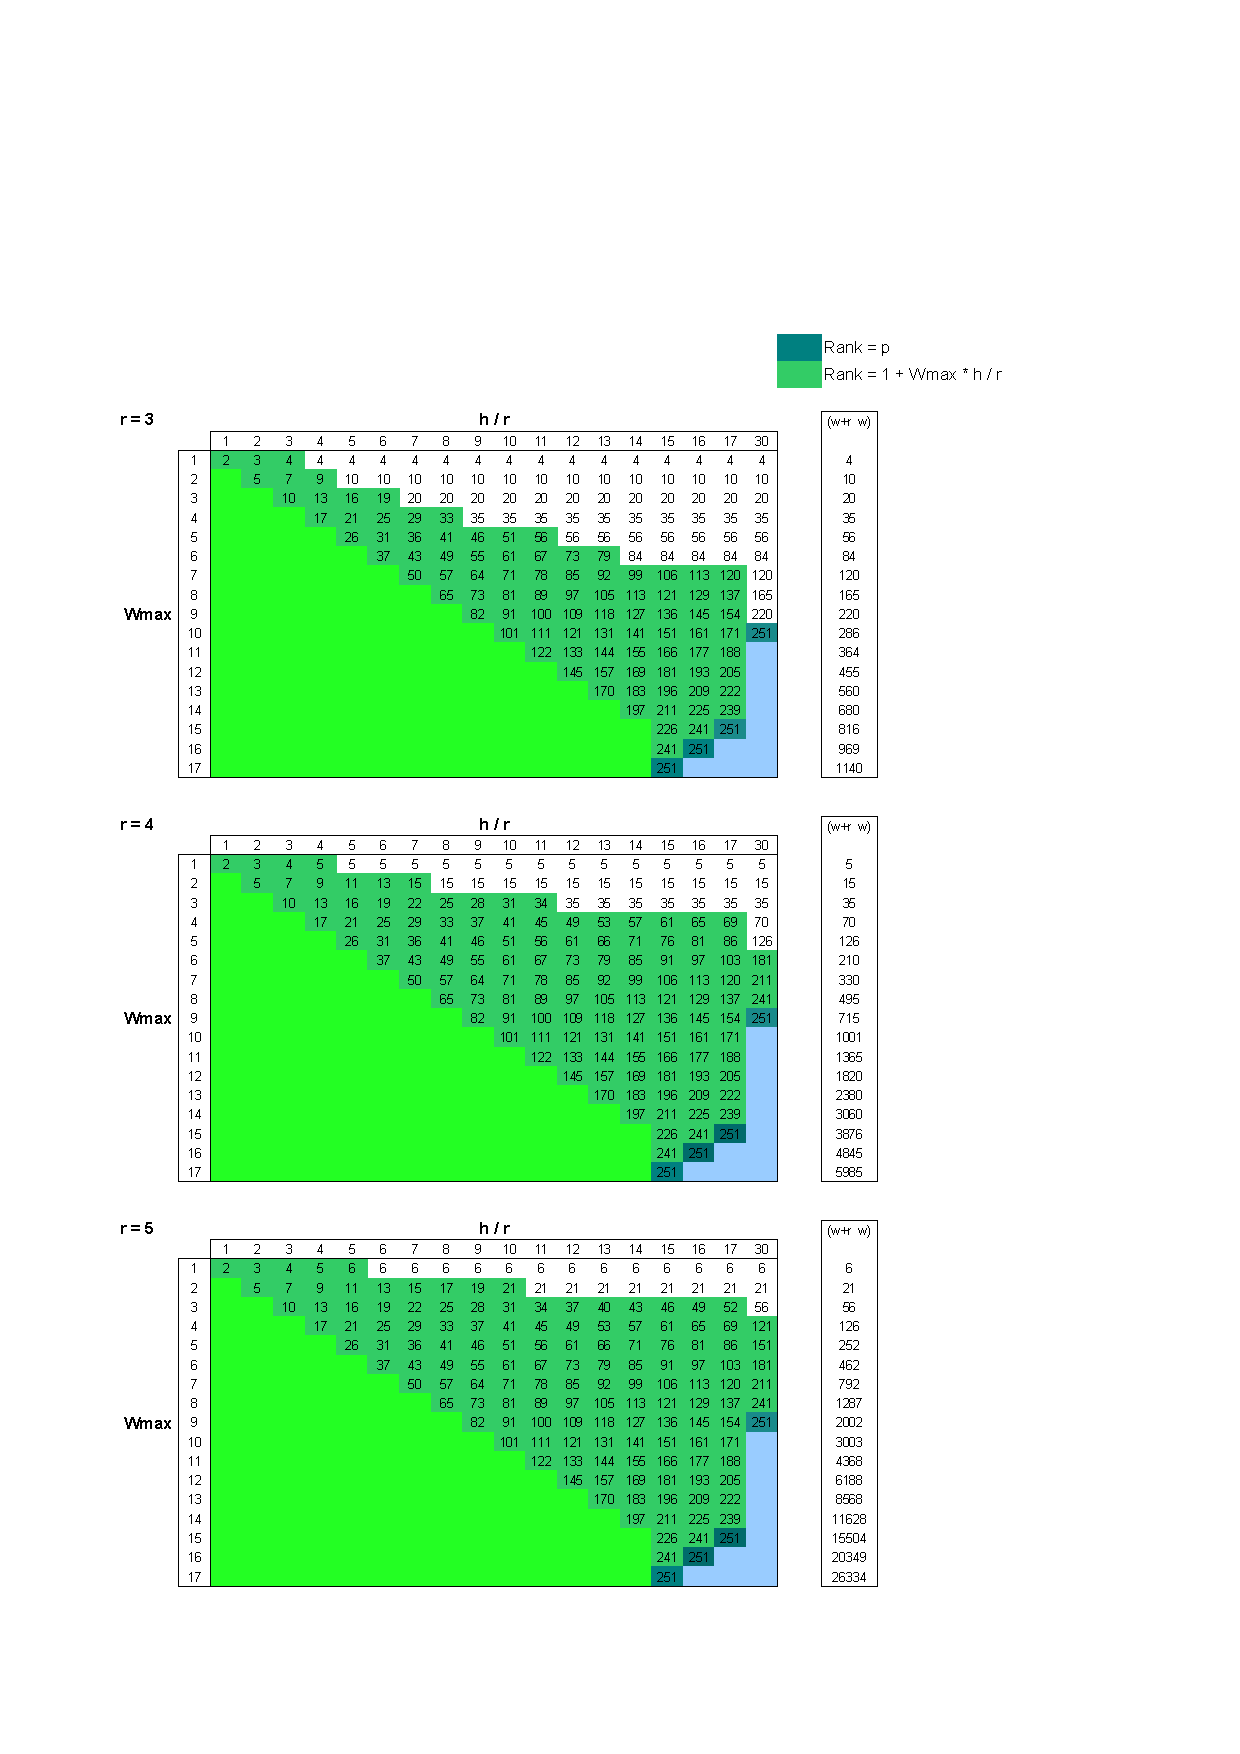
\includepdf{include/SimResults2.pdf}
\end{minipage}


\newpage
\section{Time tables}
\label{Sim:time}

\subsection{The Sidelnikov Shestakov attack}
\label{time:SS}

\begin{minipage}[H]{30cm}
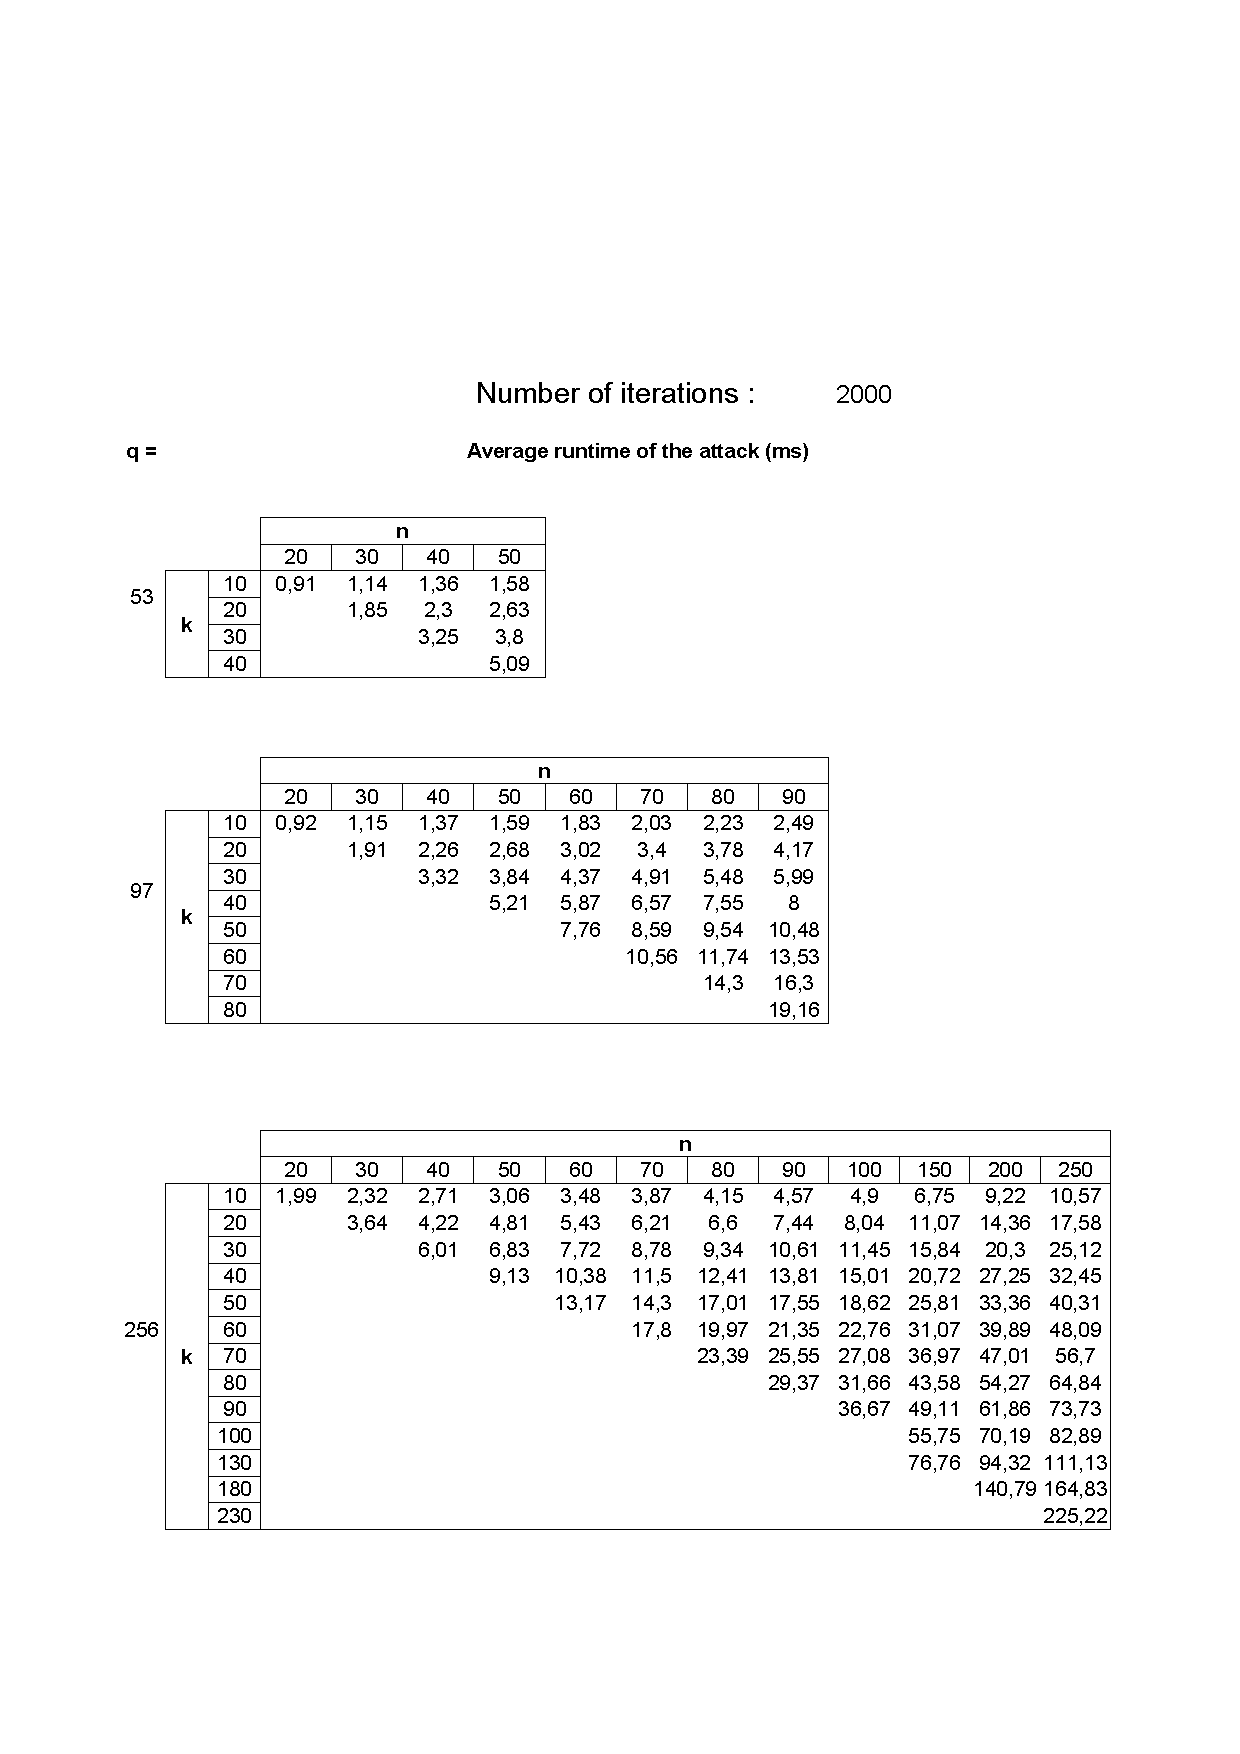
\includepdf{include/TimeTable.pdf}
\end{minipage}



\newpage
\subsection{Our attack}
\label{time:our}

We present here the results from the execution of our attack. We consider here that $g_{p^r}$ is found and we are only interested in the generation of all the possible permutations $\pi$. Each time we check that the initial permutation is indeed among the permutations generated.

The Sidelnikov-Shestakov attack itself is quite fast but the number of different possible permutations generated make this attack hard to perform on a real cryptosystem.


\begin{minipage}[H]{30cm}
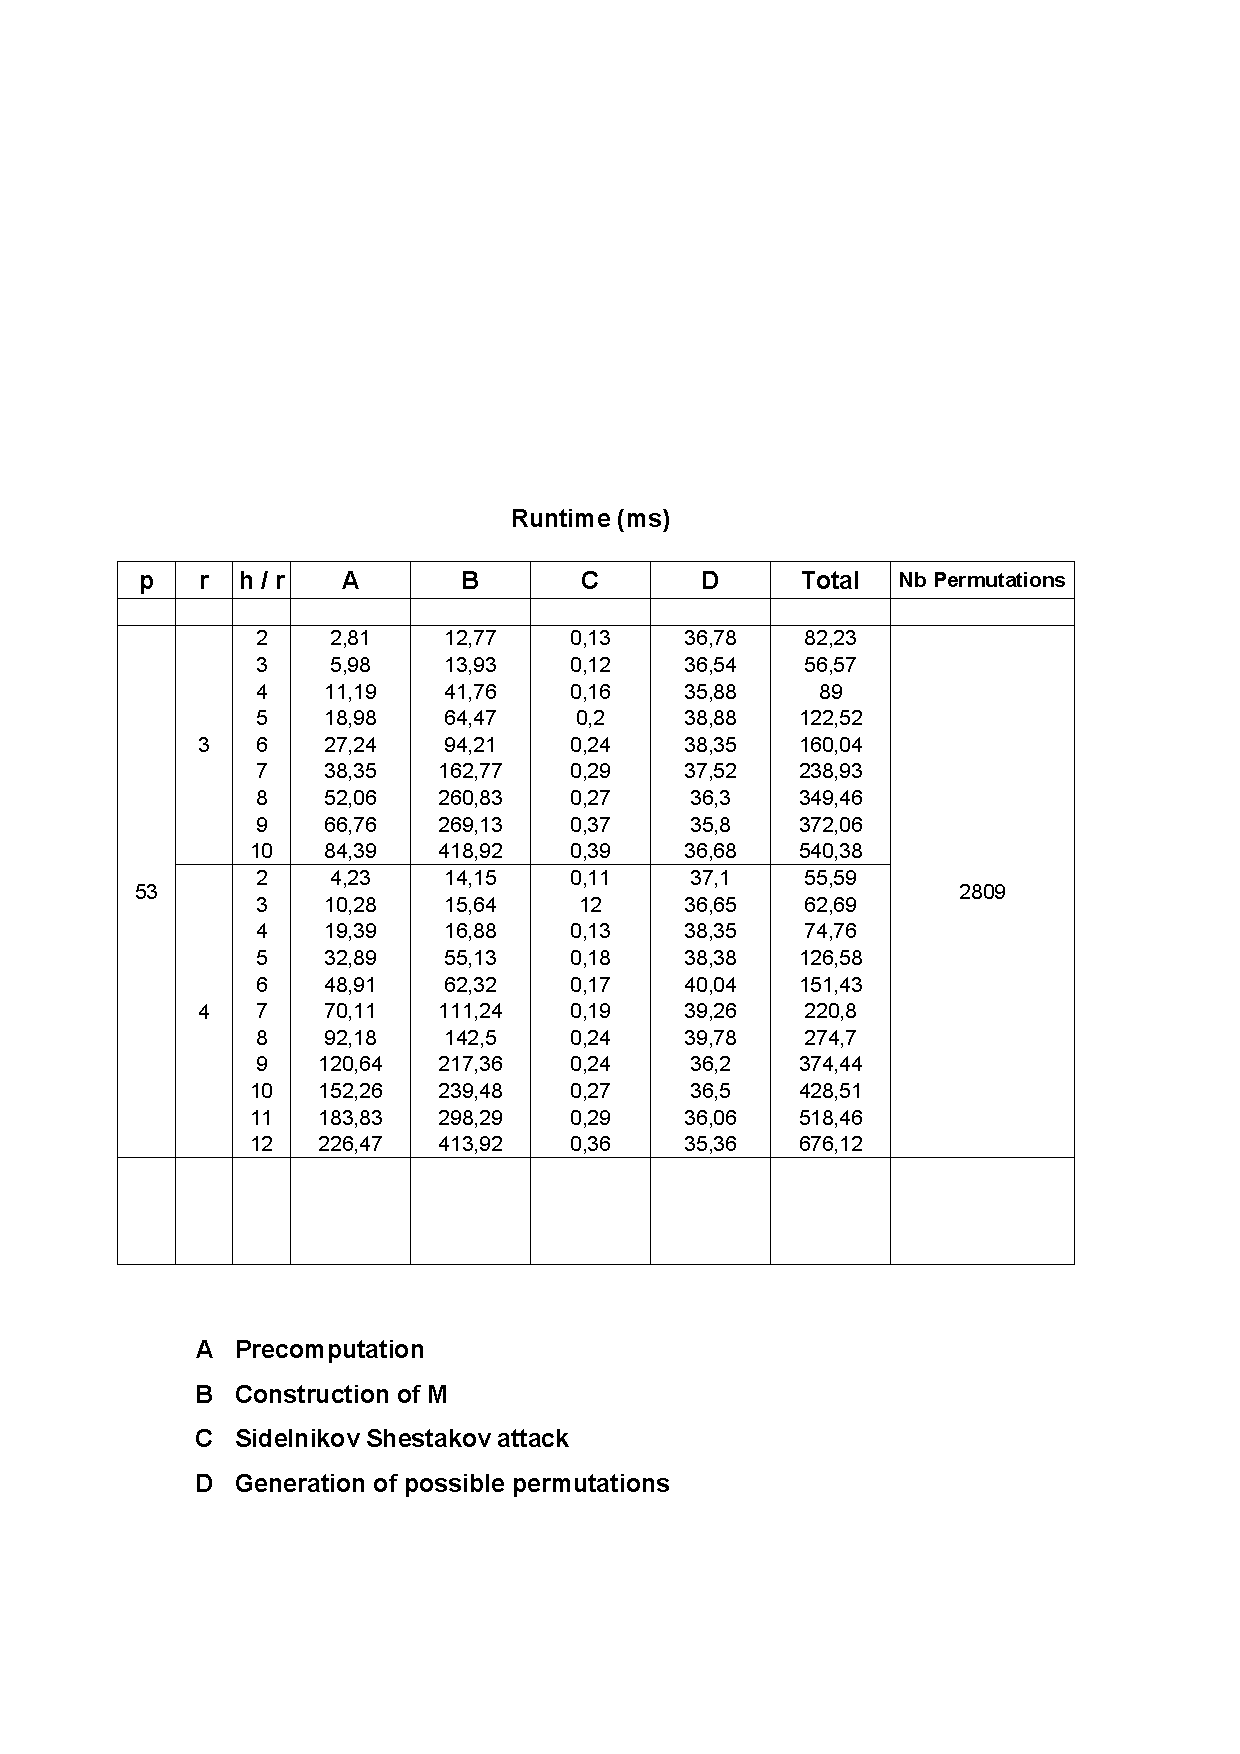
\includepdf{include/TimeTableCR.pdf}
\end{minipage}



\end{document}
